\icode{E-EME-SI-L2-261121-002}
如“顿牟掇芥”是东汉王充在《论衡·乱龙篇》中记载的摩擦起电现象，意指摩擦后的带电琥珀能吸引轻小物体。现做如下简化：在某处固定一个电荷量为\(Q\)的带正电的点电荷，在其正下方\(h\)处有一个原子。在点电荷的电场作用下，原子的负电荷中心与正电荷中心会分开很小的距离\(l\)，点电荷与原子之间产生作用力\(F\)。你可能不会求解\(F\)，但是你可以通过物理分析进行判断，关于\(F\)的表达式，可能正确的是（式中\(k\)为静电力常量）\paren[]

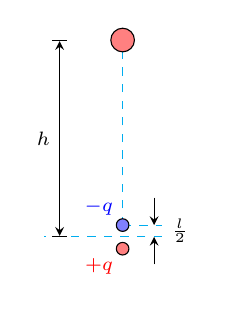
\begin{tikzpicture}[>=stealth,font=\scriptsize]
	\draw[dashed,thin,cyan] (.5,0)--(-1,0) (0,.15)--(0,2.5) (0,.15)--(.5,.15);
	\draw[fill=red!50] (0,-.15)node[below left,red]{\( + q\)} circle(.08) (0,2.5) circle(.15);
	\draw[fill=blue!50] (0,.15)node[above left,blue]{\( - q\)} circle(.08);
	\draw[|<->|] (-.8,2.5)--node[left]{\(h\)}(-.8,0);
	\draw[->] (.4,.5)--(.4,.15);
	\draw[->] (.4,-.35)--(.4,0);
	\node at(.5,.075)[right]{\(\frac{l}{2}\)};
\end{tikzpicture}
\begin{choices}
	\item \(F = 0\)
	\item \(F = \dfrac{kQq}{l^2}\)
	\item \(F = \dfrac{2kQq}{h^2}\)
	\item \(F = \dfrac{2kQql}{h^3}\)
\end{choices}
\begin{answer}
	D\qquad 提示：\(F = \dfrac{2kQqhl}{(h^2 - \frac{l^2}{4})^2}\)
\end{answer}